\documentclass[compress,red]{beamer}
\usepackage[utf8]{inputenc}
\usepackage{ucs}
\usepackage{amsmath}
\usepackage{amsfonts}
\usepackage{amssymb}
\usepackage[russian]{babel}
\usepackage{graphicx}
\usepackage{wrapfig}

\usepackage{tikz}
\usepackage{verbatim}

\usepackage{color}
\usepackage{xcolor}
\usepackage{listings}

\usepackage{caption}
\DeclareCaptionFont{white}{\color{white}}
\DeclareCaptionFormat{listing}{\colorbox{gray}{\parbox{\textwidth}{#1#2#3}}}
\captionsetup[lstlisting]{format=listing,labelfont=white,textfont=white}

\usetikzlibrary{calc,trees,positioning,arrows,chains,shapes.geometric,%
    decorations.pathreplacing,decorations.pathmorphing,shapes,%
    matrix,shapes.symbols}

\tikzset{
>=stealth',
  punktchain/.style={
    rectangle, 
    rounded corners, 
    % fill=black!10,
    draw=black, very thick,
    text width=10em, 
    minimum height=3em, 
    text centered, 
    on chain},
  line/.style={draw, thick, <-},
  element/.style={
    tape,
    top color=white,
    bottom color=blue!50!black!60!,
    minimum width=8em,
    draw=blue!40!black!90, very thick,
    text width=10em, 
    minimum height=1.5em, 
    text centered, 
    on chain},
  every join/.style={->, thick,shorten <=1pt},
  decoration={brace},
  tuborg/.style={decorate},
  tubnode/.style={midway, right=2pt},
}

\mode<presentation>

\usetheme{Warsaw}

\definecolor{Red}{rgb}{1,0,0}
\definecolor{Blue}{rgb}{0,0,1}
\definecolor{Green}{rgb}{0,1,0}
\definecolor{magenta}{rgb}{1,0,.6}
\definecolor{lightblue}{rgb}{0,.5,1}
\definecolor{lightpurple}{rgb}{.6,.4,1}
\definecolor{gold}{rgb}{.6,.5,0}
\definecolor{orange}{rgb}{1,0.4,0}
\definecolor{hotpink}{rgb}{1,0,0.5}
\definecolor{newcolor2}{rgb}{.5,.3,.5}
\definecolor{newcolor}{rgb}{0,.3,1}
\definecolor{newcolor3}{rgb}{1,0,.35}
\definecolor{darkgreen1}{rgb}{0, .35, 0}
\definecolor{darkgreen}{rgb}{0, .6, 0}
\definecolor{darkred}{rgb}{.75,0,0}

\xdefinecolor{olive}{cmyk}{0.64,0,0.95,0.4}
\xdefinecolor{purpleish}{cmyk}{0.75,0.75,0,0}

\useoutertheme[subsection=false]{smoothbars}

\title{Сервисы Google: GMail и Google Docs}
\author{ }
\date{ }

%\usecolortheme{dolphin}


\begin{document}
%%титульная страница
\maketitle
%% основные моменты

\section{GMail}
\subsection{GMail}
\begin{frame}
  \frametitle{Главная страница}
    \centerline{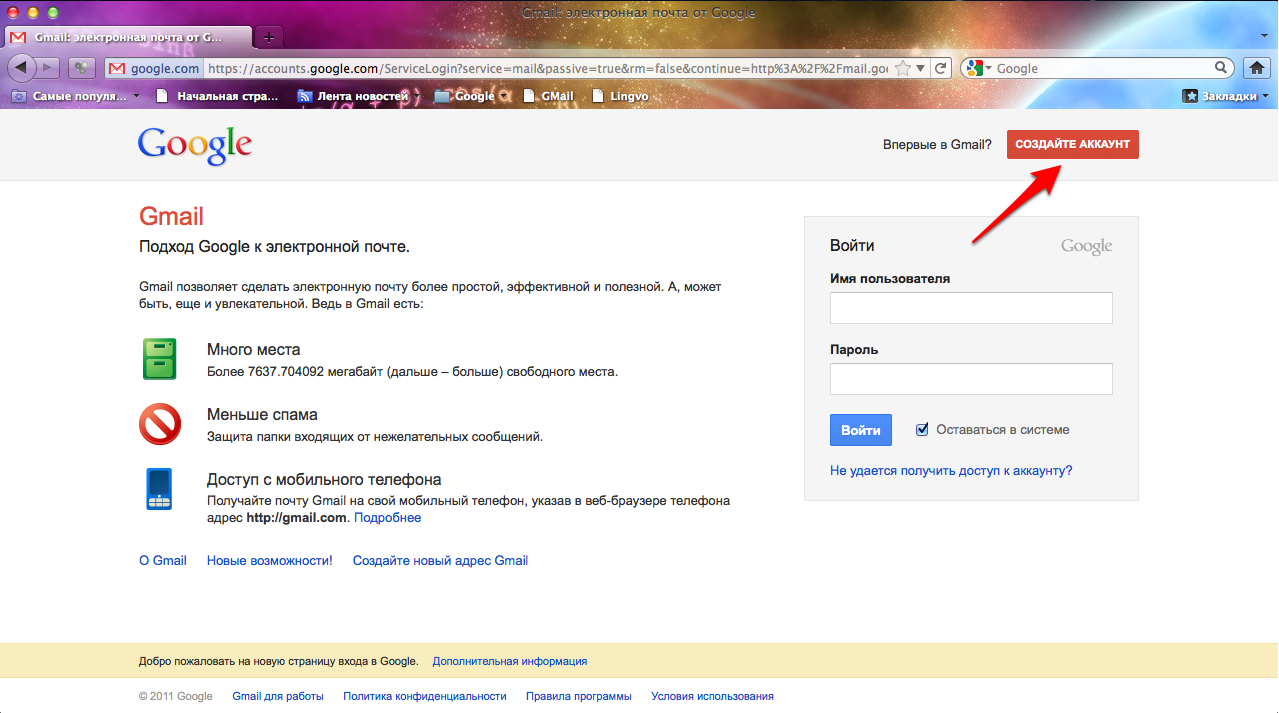
\includegraphics[width=1.0\textwidth]{images/gmail-01.png}}
\end{frame}

\subsection{GMail}
\begin{frame}
  \frametitle{Регистрация}
    \centerline{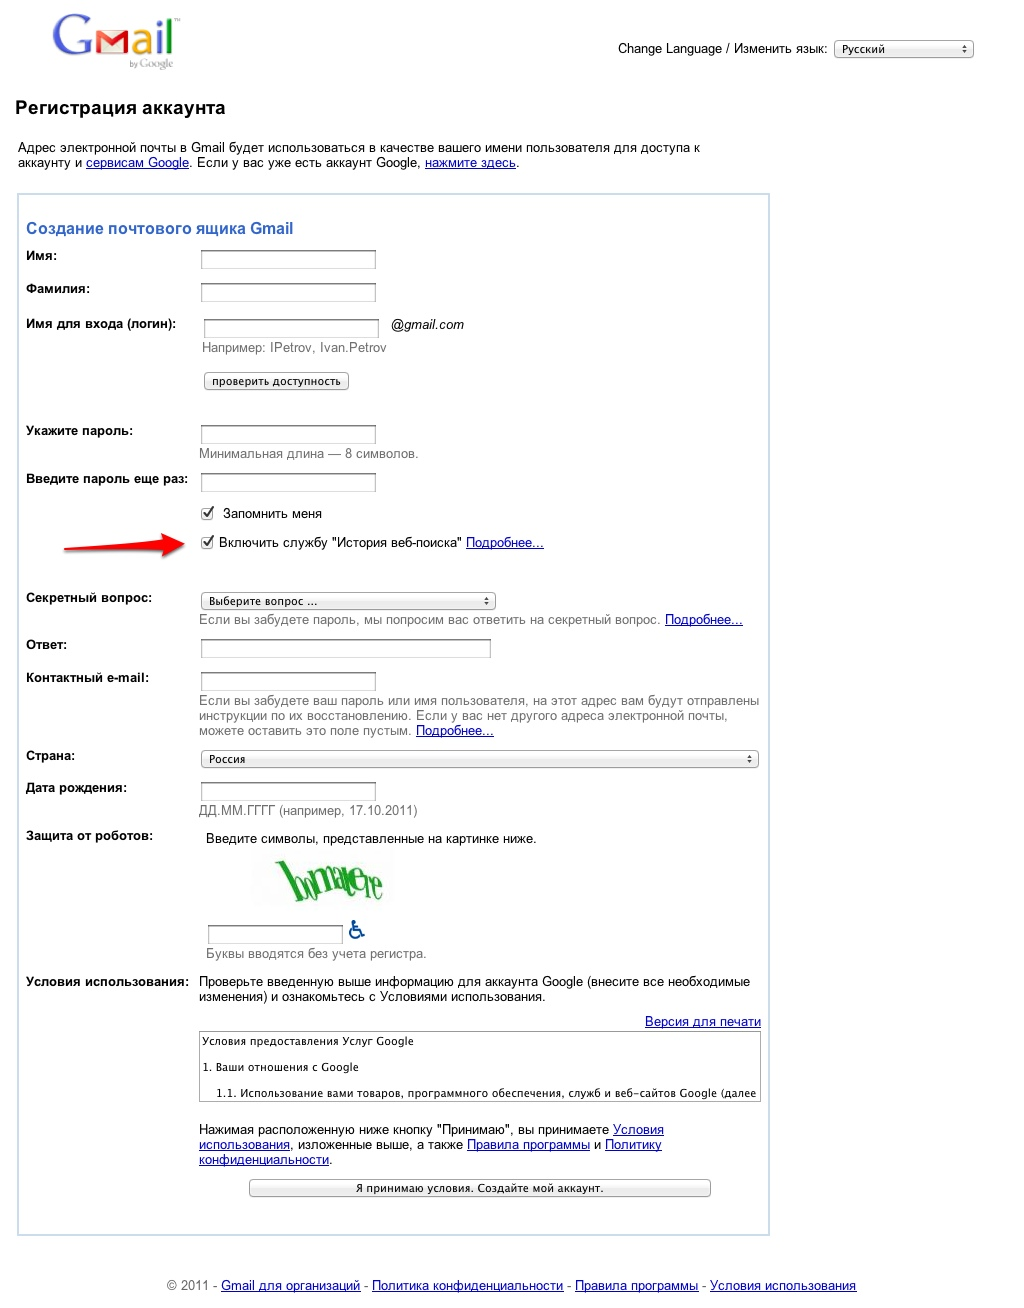
\includegraphics[width=0.5\textwidth]{images/gmail-02.png}}
\end{frame}

\subsection{GMail}
\begin{frame}
  \frametitle{Состав GMail}
    \centerline{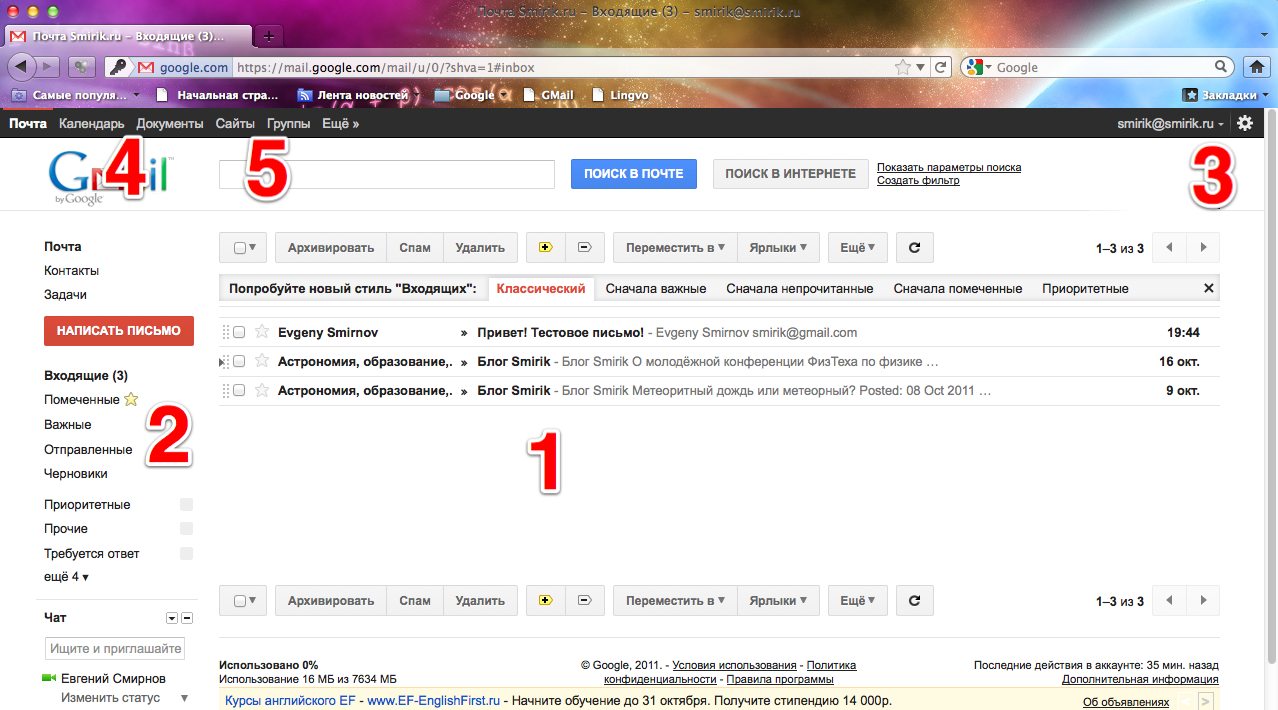
\includegraphics[width=1.0\textwidth]{images/gmail-03.png}}
\end{frame}

\subsection{Описание}
\begin{frame}[fragile]
  \frametitle{Введение}
	\begin{itemize}
	\item 1 --- центральная область, письма, настройки
	\item 2 --- ярлыки, создание письма, контакты, чат
	\item 3 --- настройки
	\item 4 --- навигация, другие сервисы
	\item 5 --- поиск
	\end{itemize}
\end{frame}

\subsection{Возможности}
\begin{frame}[fragile]
  \frametitle{Основные возможности GMail}
	\begin{itemize}
  	\item Просмотр входящих писем, разделение на приоритетные / неприоритетные. Цепочки писем.
  	\item Автоматическая фильтрация СПАМа.
  	\item Распределение писем по папкам--ярлыкам.
  	\item Автоматическая фильтрация писем по ярлыкам на основе правил.
  	\item Цветовое разделение писем.
  	\item Автоматическое сохранение черновиков.
  	\item Ведение списка контактов.
  	\item Различные темы оформления.
	\end{itemize}
\end{frame}

\subsection{Видео 1}
\begin{frame}[fragile]
  \frametitle{Видео 1}
  \begin{itemize}
    \item Здесь было видео №1.
  \end{itemize}
\end{frame}

\section{Google Docs}
\subsection{Сервисы}
\begin{frame}
  \frametitle{Google Docs}
	\centerline{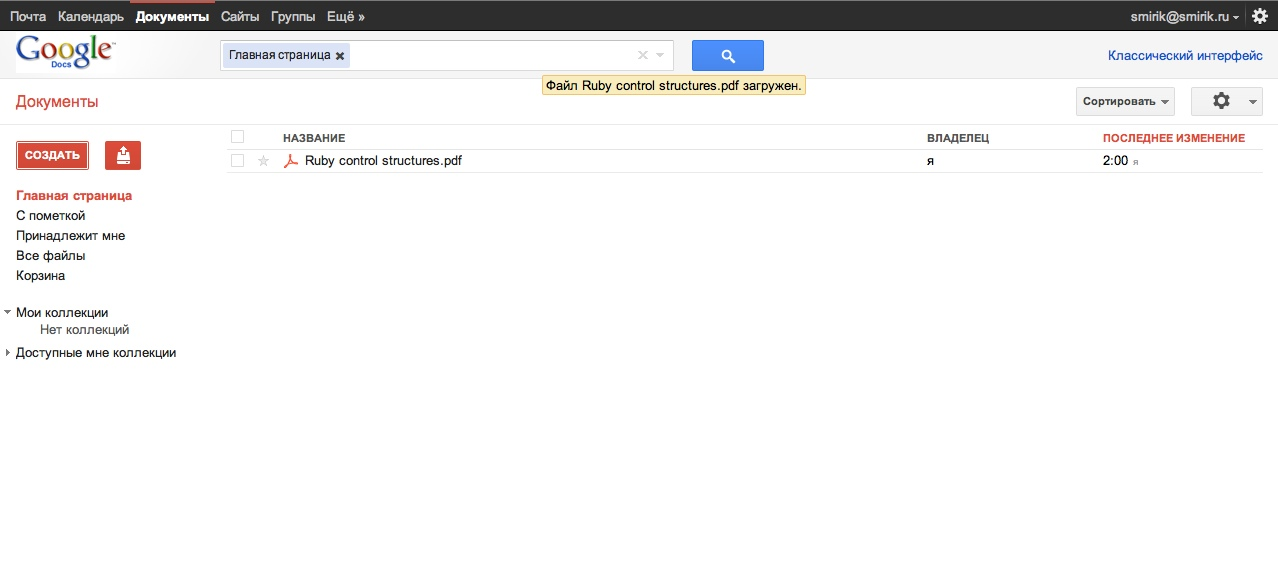
\includegraphics[width=1.0\textwidth]{images/gdocs1.jpg}}
\end{frame}

\subsection{Возможности}
\begin{frame}[fragile]
  \frametitle{Основные возможности Google Docs}
	\begin{itemize}
  	\item Создание, редактирование, импорт, экспорт офисных документов.
  	\item Возможность одновременной работы над одним документом.
  	\item Организация документов в коллекции.
  	\item Публичные коллекции (доступны нескольким пользователям).
  	\item Базовые возможности офисного пакета.
	\end{itemize}
\end{frame}

\subsection{Видео 2}
\begin{frame}[fragile]
  \frametitle{Видео 2}
  \begin{itemize}
    \item Здесь было видео №2.
  \end{itemize}
\end{frame}

\section{Задания}
\subsection{Задания}
\begin{frame}
  \frametitle{Задания}
	\begin{enumerate}
  	\item Зарегистрировать Google--аккаунт (если нет).
  	\item Отправить тестовое письмо на smirik@gmail.com.
  	\item Получить ответным письмом ссылку на Google-документ --- таблицу. Внести себя в список.
  	\item Выполнить домашнее задание по программированию (на будущую среду) в виде Google-документа. Расшарить документ для smirik@gmail.com.
  	\item В случае появления комментариев оперативно отвечать и исправлять.
	\end{enumerate}
	\begin{itemize}
	  \item Оценка приблизительно равна количеству правильно выполненных пунктов.
	\end{itemize}
\end{frame}

\subsection{References}
\begin{frame}[fragile]
  \frametitle{References}
  \begin{itemize}
    \item Все презентации доступны на http://school.smirik.ru!
    \item Вопросы, предложения, д/з: smirik@gmail.com
  \end{itemize}
\end{frame}


\end{document}